\documentclass[12pt, titlepage]{article}
\usepackage[utf8]{inputenc}
\usepackage{graphicx}
\usepackage{amsmath}
\usepackage{amssymb}
\usepackage[spanish, activeacute]{babel} %Definir idioma español
\usepackage{textcomp, gensymb}
\usepackage[spanish]{babel}
\selectlanguage{spanish}
\usepackage[utf8]{inputenc}
\usepackage[font=small,labelfont=bf]{caption}

\usepackage[utf8]{inputenc} %Codificacion utf-8
\graphicspath{ {./imagenes} }
\usepackage{geometry}
 \geometry{
 a4paper,
 total={170mm,257mm},
 left=20mm,
 top=20mm,
 }






\begin{document}
\title{Trabajo práctico. Análisis de Circuitos}
\author{Adrián Romero}
\date{1er cuatrimestre, año 2020}
\maketitle

\tableofcontents


\maketitle

\newpage
\section{Objetivo}

El objetivo del presente trabajo pr'actico es estudiar y dise'nar un filtro a partir de una función de transferencia dada. Se hallarán los polos y ceros de la transferencia, los parámetros $w_0$ y $Q$ sabiendo que la función de transferencia del filtro es: 

\begin{center}
    $
    \frac{s^2 \cdot 2,527 \cdot 10^9}
    {s^4 + s^3 \cdot 7,153 \cdot 10^4 + 
     s^2 \cdot 2,558 \cdot 10^9  +
     s \cdot 1,13\cdot 10^{12} +
     2,494 \cdot 10^{14} }
$
\end{center}

Luego se procederá a hallar y analizar las respuesta al impulso, al escal'on y a se'nales cuadradas y senoidales, adem'as de los diagramas de Bode de magnitud y fase del filtro.

Posteriormente se dise'nará un filtro que tenga la transferencia asignada, a partir de valores normalizados de resistencias y capacaitores y se comparar'an sus respuestas con las respuestas esperadas a partir del an'alisis anteriormente mencionado.

Finalmente se buscar'an las respuestas anal'iticas a las se'nales anteriores.

\section{Análisis del filtro a partir de la función de transferencia}
    \subsection{Análisis del tipo filtro}
    \subsubsection{Orden}
    
    A partir de la función de transferencia podemos ver que es un filtro de orden 4. Esto se deduce del hecho de que el denominador sea un polinomio de grado 4 y por lo tanto habrá cuatro polos.
    
    \subsubsection{Tipo}
    
    Para poder decir si es un filtro de tipo pasabajo, pasalto, rechazabanda o pasabanda analizamos el comportamiento del filtro (a partir de analizar la función de transferencia) para frecuencias altas y para frecuencias bajas. \vspace{5mm}
    
    Para frecuencias altas hacemos tender s a infinito:  $\lim_{s \to \infty} H(s)$ = 0
    
    Esto es evidente pues el grado del polinomio en el denominador es mayor que el del numerador. \vspace{5mm}
     
    Para frecuencias bajas hacemos tender s a 0: $\lim_{s \to 0} H(s)$ = 0
    
    Dado que tanto para frecuencias altas como para frecuencias bajas la transferencia resulta 0, deducimos que estamos en presencia de un filtro pasabanda. 
    
    \subsection{Calculo de ceros, polos, $w_0$ y Q}
    \subsubsection{Ceros}
    
    Dado que el numerador de la transferencia es: $s^2 \cdot 2,527 \cdot 10^9$, se observa fácilmente que hay un cero de orden 2 en s=0.
    
    \begin{center}
        $z_1 = z_2 = 0$
    \end{center}
    
    \subsubsection{Polos}
    Para el calculo de polos buscamos aquellos valores que anulan el denominador de la transferencia, es decir resolvemos la ecuación:
 \begin{center}
   $ s^4 + s^3 \cdot 7,153 \cdot 10^4 + 
     s^2 \cdot 2,558 \cdot 10^9  +
     s \cdot 1,13\cdot 10^{12} +
     2,494 \cdot 10^{14} = 0$
\end{center}   

    Las soluciones obtenidas con Matlab fueron:
    \begin{center}
    $ p_{a} = \sigma_a + w_{da}j =  -35542.74 + 35538.93j$
    
    $\overline{p_{a}}= \sigma_a - w_{da}j =-35542.74 - 35538.93j$
    
    $p_{b} = \sigma_b + w_{db}j =-222.25 + 222.08j$
    
    $\overline{p_{b}} = \sigma_b - w_{db}j =-222.25 - 222.08j$
    \end{center}
    
    Se observa que son dos pares de polos complejos conjugados.

    \subsubsection{$w_0$ y Q}
    A partir de los cuatro polos obtenidos en el apartado anterior podemos descomponer el denominador de la transferencia en el producto de dos polinomios de grado 2. 
    
    \begin{center}
    $(s-p_{a})(s-\overline{p_{a}})(s-p_{b})(s-\overline{p_{b}})$ = $(s^2 - 2Re(p_{a}) + |p_{a}|^2)(s^2 - 2Re(p_{b}) + |p_{b}|^2)$
    \end{center}
    
    Luego, se calculan $w_a, Q_a$ y $w_b, Q_b$ las frecuencias naturales y los factores de calidad asociados a los polos $p_{a}$ y $p_{b}$ respectivamente a partir de la forma general de las transferencias de segundo orden: $s^2 + s \cdot \frac{w_i}{Q_i} + {w_i}^2$. Obtuvimos los siguientes resultados: 
    \begin{center}
    $w_a$ =  $50262.33\frac{rad}{s}$ \hspace{7mm}
    $Q_a$ =    0.70\\
    $w_b$ =  $314.19\frac{rad}{s}$ \hspace{7mm}
    $Q_b$ =    0.70\\
    \end{center}
    
    Como era de esperarse, pues en la sección anterior obtuvimos pares de polos complejos conjugados, $Q_{a}$ y $Q_{b}$ cumplen que: 
    
    \begin{center}
        $Q_{a} > \frac{1}{2} \hspace{6mm} Q_{b}>\frac{1}{2}$
    \end{center}
    
    Y por lo tanto la respuesta al escal'on sera de tipo suma de se'nales subamortiguadas:
    
    \begin{center}
        $e^{-\frac{t}{\tau_{1}}}(Asen(w_{d1}) + Bcos(w_{d1}))+e^{-\frac{t}{\tau_{2}}}(Csen(w_{d2}) + Dcos(w_{d2})) $
    \end{center}
    
    Donde:
    
    \begin{center}
        $w_{da} = w_a\sqrt{1-\frac{1}{4Q_a^2}} = 35176.3 \simeq Im(p_a) \hspace{8mm} w_{db} = w_b\sqrt{1-\frac{1}{4Q_b^2}} = 219.9 \simeq Im(p_b)$\\
        \vspace{3mm}
        $\tau_1 = \frac{1}{-\sigma_1} = 4.5\cdot 10^{-3} \hspace{8mm} \tau_2 = \frac{1}{-\sigma_2} = 2.8\cdot 10^{-5} $
    \end{center}
    
    Donde los valores son aproximadamente los esperados, probablemente debido a redondeos que realiza Matlab al encontrar los polos. 
    
    Finalmente, dado que el filtro a analizar es un pasabanda, la frecuencia natural $w_0$ resultará la media geométrica entre $w_a$ y $w_b$, es decir, $w_0$ = $\sqrt{ w_a w_b}$
    \begin{center}
    $w_0$ =  $3973.96\frac{rad}{s}$\\
    \end{center}
    
    
    \newpage
    
    \subsection{Diagramas de Bode}
    Utilizando la función \emph{Bode()} de Matlab hallamos la respuesta en frecuencia del filtro representados en los diagramas de Bode para magnitud en dB y fase en grados.
    \subsubsection{Magnitud}
    Observamos que tal como se predijo la máxima ganancia en magnitud se alcanza en $w_0$ = $3973.96\frac{rad}{s}$. La ganancia es de aproximadamente 0dB para $w_0$ lo que indica una ganancia unitaria en tensión. 
    
    \begin{figure}[!htb]
     \includegraphics[width= 13.65cm, height=6.5cm]{imagenes/bode_magnitud.png}
     \centering
     \caption{Diagrama de Bode de magnitud - $w_0$}
    \end{figure}
    
    Observamos que para $w_a =  50262.33\frac{rad}{s}$ y $w_b =  314.19\frac{rad}{s}$ la ganancia en magnitud es aproximadamente la misma: -3dB. Esto indica una relación del 70\% entre la tensión de salida y la tensión de entrada. Esto se debe a que $20log(Q_a) = 20log(Q_b) = 20log(0.7)$ = -3dB.
    
    Adem'as se puede observar que las pendientes de subida y de bajada en magnitud son de $\pm40\frac{dB}{dec}$ donde la subida se debe al cero doble en 0, la estabilizacion al polo complejo de $314,19\frac{rad}{s}$ y la bajada al polo de $50262.33\frac{rad}{s}$
    \begin{figure}[!htb]
     \includegraphics[width= 13.65cm, height=6.5cm]{imagenes/bode_magnitud2.png}
     \centering
     \caption{Diagrama de Bode de magnitud - $w_a$ y $w_b$}
    \end{figure}
    
    \newpage
    
    \subsubsection{Fase}
    \begin{figure}[!htb]
     \includegraphics[width= 16cm, height=6.5cm]{imagenes/bode_fase.png}
     \centering
     \caption{Diagrama de Bode de fase}
    \end{figure}
    
    Podemos ver que como la transferencia tiene un cero doble en $s=0$, la fase inicial resulta $2 \cdot90\degree = 180\degree$
    
    Además, el cambio de fase entre que ocurre entre las frecuencias una década antes de $w_{a} = 314.19\frac{rad}{s}$ y una década después de $w_{a}$ es de $180\degree$, con una pendiente de $\frac{-90\degree}{dec}$, pasando por $90\degree$ en la frecuencia $w_a$, tal como es esperado para los polos complejos conjugados. Lo mismo sucede para $w_b = 50262.33\frac{rad}{s}$ excepto que a esa frecuencia la fase es de $-90\degree$.
    
    \subsection{Respuesta al escalón}
    La respuesta al escalón del sistema se puede hallar buscando la transformada inversa de laplace de $\frac{H(s)}{s}$
    
    
    Utilizando la función \emph{ilaplace()} de Matlab se obtuvo la siguiente respuesta al escalón: 
    \begin{center}
     $- exp(-35544.0t)cos(35544.0t)(0.5064 - 0.5002i) -$ \\ $exp(-35544.0t)cos(35544.0t)(0.5064 + 0.5002i) -$ \\ $exp(-35544.0t)sin(35544.0t)(0.5002 + 0.5064i) -$ \\ $exp(-35544.0t)sin(35544.0t)(0.5002 - 0.5064i) +$ \\ $exp(-222.2t)cos(222.1t)(0.5064 - 0.5005i) +$ \\ $exp(-222.3t)cos(222.1t)(0.5065 + 0.5005i) -$\\ $exp(-222.2t)sin(222.1t)(0.5005 + 0.5064i) -$\\ $exp(-222.3t)sin(222.1t)(0.5005 - 0.5064i)$     
    \end{center}
    
    Agrupando los términos semejantes y aproximando valores parecidos logramos obtener una ecuación simplificada de la respuesta al escalón:
    \begin{center}
        $-e^{-35544t}(cos(35544t)+sin(35544t)) + e^{-222.2t}(cos(222.2t) - sin(222.2t))$
    \end{center}
        
    
    Procedemos a graficar esta expresión y compararla con aquella que otorga la función \emph{step()} de Matlab:

    \newpage
    
    \begin{figure}[!htb]
     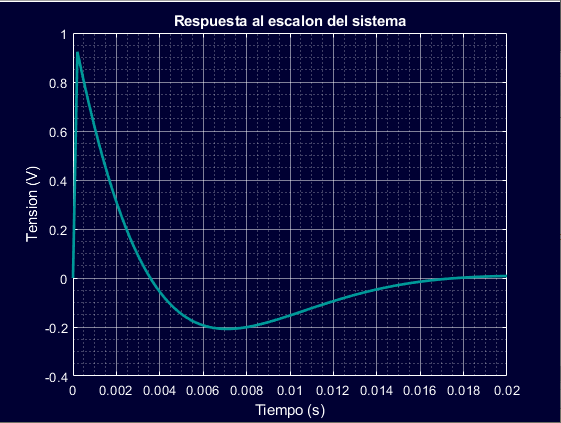
\includegraphics[scale = 0.9]{imagenes/escalon_ilaplace.png}
     \centering
     \caption{Respuesta al escalón hallada con \emph{ilaplace()}}
    \end{figure}
    
    \begin{figure}[!htb]
     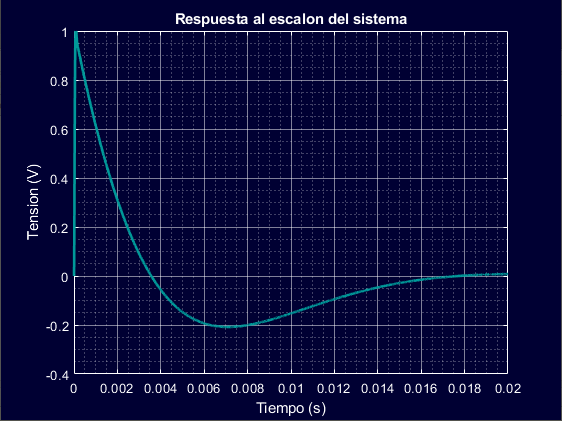
\includegraphics[scale = 0.9]{imagenes/escalon_step.png}
     \centering
     \caption{Respuesta al escalón hallada con \emph{step()}}
    \end{figure}

    \newpage

    Observamos que ambas respuestas al escalón halladas son muy similares. Sin embargo, es posible apreciar que en la respuesta hallada con \emph{step()} logra alcanzar un valor máximo mayor que el hallado con \emph{ilaplace()}. A pesar de esto, consideramos que la respuesta al escalón hallada con \emph{ilaplace()} es representativa del comportamiento del filtro.

    
    La constante de tiempo $\tau$ para este circuito puede obtenerse comparando los inversos de los coeficientes de las exponenciales de la respuesta al escalón obtenida: 
    
     \begin{center}
        $\tau_1 = \frac{1s}{222.2} = 0.0045s$ \hspace{5mm} $\tau_2 = \frac{1s}{35544} = 0.000028s$ 
    \end{center}
    
    Estos valores son los que esperábamos de acuerdo al análisis hecho en la secci'on anterior.
    
    Dado que $\tau_1 >> \tau_2$ es evidente que la respuesta al escalón se amortiguara casi completamente en un tiempo de: $4\tau_1 = 0.018s$ como se puede ver en las figuras 4 y 5.
    
    Además observamos que durante los primeros $4\tau_2 = 0.000112s$ de tiempo se puede apreciar el efecto de la suma de ambas exponenciales al mismo tiempo y por eso la respuesta alcanza un valor mas alto. Luego de este tiempo solo es posible apreciar el efecto de una de las exponenciales pues la otra estará amortiguada.
    
    Si relacionamos $w_da$ con $4\tau_1$ podremos estimar cuantos periodos de las senoidales amortiguadas podremos ver:
    
    \begin{center}
        $\frac{\frac{w_{da}}{2\pi}}{4\tau_1}$ = 1.57
    \end{center}
    
    La figura anterior se corresponde con este resultado pues solo podemos ver aproximadamente 1 periodo de senoidal antes de su amortiguamiento.
    
    Debido a que el filtro es un pasabanda podemos ver que en el flanco del escalón la respuesta en tensión es nula. Esto se debe a que el flanco del escalón esta asociado con las altas frecuencias y un filtro pasabanda las filtra. 
    
    Además podemos observar que luego de que transcurre el transitorio - un tiempo de $4\tau = 0.018s$ - la tensión de la respuesta al escalón es también nula. Esto se debe a que un filtro pasabanda también filtra las bajas frecuencias que se asocian con el régimen permanente o continuo. 
    
   
    
    \subsection{Respuesta al impulso} 
    Buscamos la respuesta al impulso del sistema a traves de la antitransformada de Laplace de la funcion de transferencia $H(s)$. Nuavmente utilizamos \emph{ilaplace()} y obtuvimos:
    \begin{center}
    $exp(-35544.0*t)*cos(35544.0*t)*(223.7 - 35777.0i) + $\\ $exp(-35544.0*t)*cos(35544.0*t)*(223.7 + 35777.0i) + $\\ $exp(-35544.0*t)*sin(35544.0*t)*(35777.0 + 223.7i) + $\\ $exp(-35544.0*t)*sin(35544.0*t)*(35777.0 - 223.7i) - $\\ $exp(-222.2*t)*cos(222.1*t)*(223.7 + 1.232i) - $\\
    $exp(-222.3*t)*cos(222.1*t)*(223.7 - 1.231i) -  $\\
    $exp(-222.2*t)*sin(222.1*t)*(1.232 - 223.7i) -  $\\ 
    $exp(-222.3*t)*sin(222.1*t)*(1.231 + 223.7i)$ 
    \end{center}
    
    Simplificando logramos obtener: 
     \begin{equation}
        e^{-35544t}(447.4cos(35544t) + 71554sin(35544t)) -  e^{-222.2t}(447.4cos(222.2t) + 2.462sin(222.2t))
    \end{equation}

    \newpage
    
    Graficando esta respuesta y la obtenida con la función \emph{impulse()} de Matlab:
    
    \begin{figure}[!htb]
     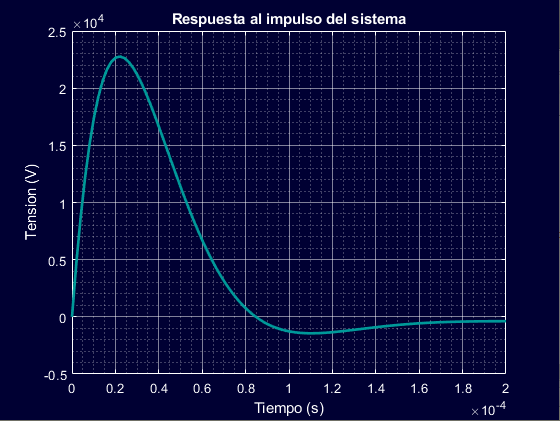
\includegraphics[scale = 0.9]{imagenes/impulso_ilaplace.png}
     \centering
     \caption{Respuesta al impulso hallada con \emph{ilaplace()}}
    \end{figure}
    
    \begin{figure}[!htb]
     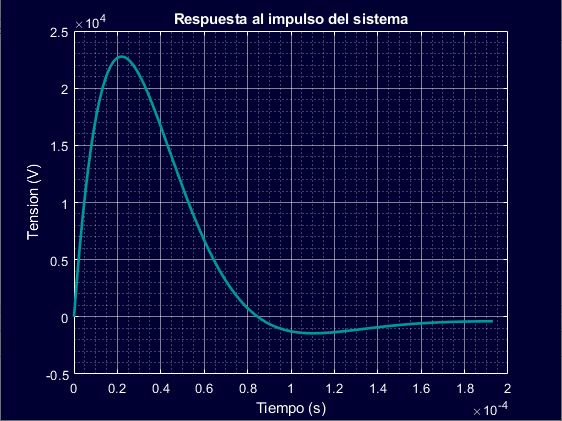
\includegraphics[scale = 0.9]{imagenes/impulso_impulse.png}
     \centering
     \caption{Respuesta al impulso hallada con \emph{impulse()}}
    \end{figure}

    No se observan diferencias apreciables entre las respuestas al impulso halladas.
    
    \subsection{Comparación entre la respuesta al impulso y la respuesta al escalón}
    Para comparar la respuesta al impulso y al escalón se graficaron ambas funciones en el intervalo de tiempo [0, 0.2e-4]. Además se reescaló la respuesta al escalón multiplicándola por un factor de 2e4.
    
     \begin{figure}[!htb]
     \includegraphics[scale = 0.9]{imagenes/comparacion_impulso-escalon(2e4escalado).png}
     \centering
     \caption{Respuesta al impulso en turquesa, respuesta al escalón -reescalada- en rojo}
    \end{figure}
    
    Realizamos las siguientes observaciones:
    
    \begin{itemize}
        \item Cuando la respuesta al impulso es positiva, la respuesta al escalón es creciente.
        \item Cuando la respuesta al impulso es negativa, la respuesta al escalón es decreciente.
        \item Cuando la respuesta al impulso es cero -indicado en la figura-, la respuesta al escalón alcanza un máximo.
        \item Cuando la respuesta al impulso tiene un máximo o un mínimo, la respuesta al escalón cambia su concavidad.
    \end{itemize}
    
    
    Esto es coherente pues la respuesta al impulso es la derivada de la respuesta al escalón.

    \subsection{Respuesta a se'nales cuadradas}
    Graficaremos ahora las respuestas del filtro a las se'nales cuadradas de frecuencias: $f_0$ = $\frac{w_0}{2\pi}$ = 632.47hZ, $10 \dot f_0$ = 6324.47hZ y $\frac{f_0}{10}$ = 63.247hZ. En cada uno de los gráficos se indica en rojo la se'nal que produce la respuesta, indicada en turquesa.

    \newpage
    
    \subsubsection{Respuesta a se'nal cuadrada de $f_0 = \frac{w_0}{2\pi}$ }
      \begin{figure}[!htb]
     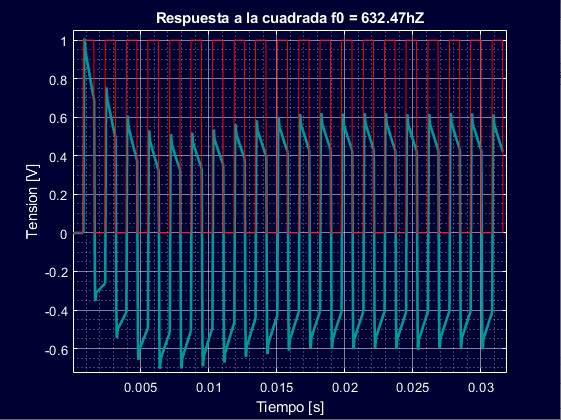
\includegraphics[scale = 0.65]{imagenes/cuadrada_f0.png}
     \centering
     \caption{Respuesta a la cuadrada de 632.47hZ en turquesa, se'nal cuadrada en rojo (20 periodos)}
    \end{figure}
    
    \begin{small}
     Observamos que luego de 0.018s ($4\tau$) la respuesta a la se'nal cuadrada de $f_0$ se estabiliza. Adem'as observaremos que en cada ventana de tiempo en el que la cuadrada est'a en el valor 1V, la respuesta es c'omo una respuesta al escal'on. Dependiendo de la frecuencia de la cuadrada se ver'a m'as o menos amortiguamiento como podremos observar en las siguientes respuestas. En particular para esta se'nal cuadrada el tiempo de amortiguamiento $4\tau > \frac{T_{cuad}}{2} = 0.00079$ y por lo tanto no se podr'a notar el amortiguamento en el semiper'iodo de cuadrada.
    \end{small}
   
    
    \subsubsection{Respuesta a se'nal cuadrada de $10 f_0 = 10\frac{w_0}{2\pi}$ }
    
      \begin{figure}[!htb]
     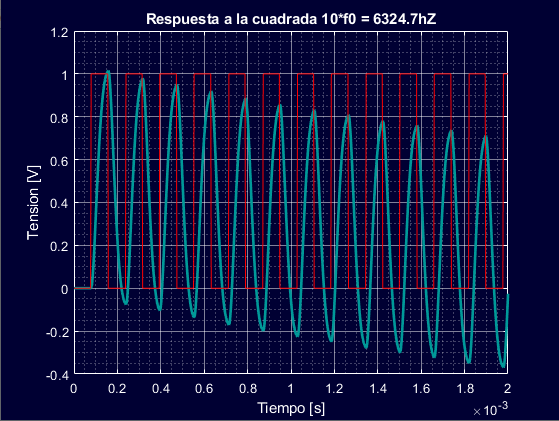
\includegraphics[scale = 0.65]{imagenes/cuadrada_10f0.png}
     \centering
     \caption{Respuesta a la cuadrada de 6324.7hZ en turquesa, se'nal cuadrada en rojo (12 periodos)}
    \end{figure}
    
    \begin{small}
        Podemos observar que cuando la frecuencia de la se'nal cuadrada es elevada, su periodo disminuye y por lo tanto le da menos tiempo al filtro a amortiguarse. 
    
    Comparando el tiempo de amortiguamiento del filtro $4\tau = 0.018s$ con el semiperiodo de la cuadrada $\frac{T_{cuad}}{2} = 0.00079s$ podemos observar que $\frac{T_{cuad}}{2} << 4\tau$ y por lo tanto no podremos notar el amortiguamiento. 
    \end{small}
    


    
    \subsubsection{Respuesta a se'nal cuadrada de $\frac{f_0}{10} = \frac{1}{10}\frac{w_0}{2\pi}$}
    
     \begin{figure}[!htb]
     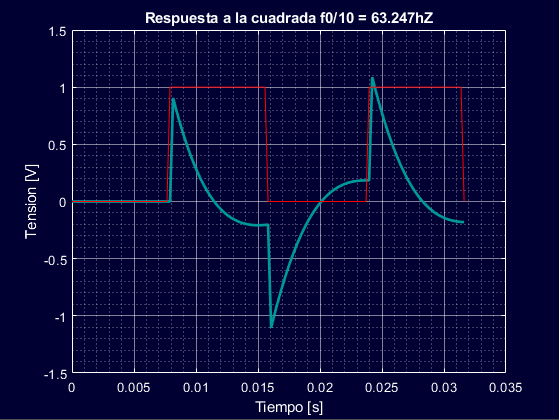
\includegraphics[scale = 0.75]{imagenes/cuadrada_f0_10.png}
     \centering
     \caption{Respuesta a la cuadrada de 63.247hZ en turquesa, se'nal cuadrada en rojo (2 periodos)}
    \end{figure}
    
    El semiperiodo de la cuadrada para este caso es:  $\frac{T_{cuad}}{2} = 0.0079$
    En este caso observamos que $\frac{T_{cuad}}{2} < 4\tau$. Por lo que si bien no veremos llegar a amortiguarse la respuesta en un semiperiodo si podremos ver mas amortiguamiento que en el caso anterior. De hecho podemos ver que en las ventanas de 0.0079s de la cuadrada, el filtro responde exactamente como los primeros 0.0079s de la respuesta al escalón.

    \subsubsection{Respuesta a se'nal cuadrada de $1000f_0$}
    
     \begin{figure}[!htb]
     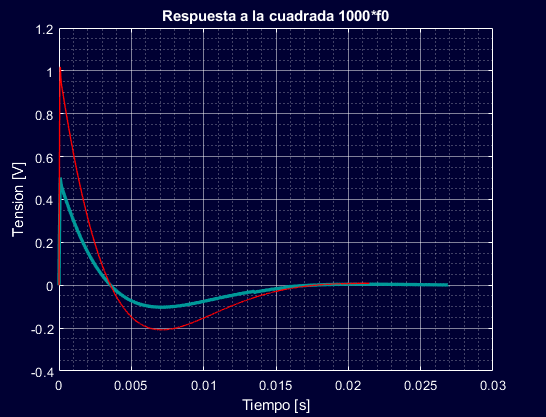
\includegraphics[scale = 0.75]{imagenes/respuesta_cuadrada_1000f0.png}
     \centering
     \caption{Comparación respuesta cuadrada 1000f0 en turquesa y respuesta al escalón en rojo}
    \end{figure}
    
    Se puede observar que la respuesta a la se'nal cuadrada se comporta como si fuera una respuesta a un escalón de amplitud $\frac{1}{2}$. 
    
    Una forma de explicar esto es mediante la descomposición en serie de Fourier de una se'nal cuadrada de frecuencia f:
    \begin{center}
        $x_{sq}(t) = V_{medio} + \frac{4}{\pi}\sum_{k_{impar}}^{\infty} \frac{sen(2\pi kft)}{k}$
    \end{center}
    
    Observamos que se puede descomponer en una suma infinita de se'nales sinusoidales.
    
    En particular para una se'nal cuadrada de valor medio $\frac{1}{2}$ y frecuencia $1000f_0$ la se'nal puede escribirse:
     \begin{center}
        $x_{sq}(t) = \frac{1}{2} + \frac{4}{\pi} (\frac{sen(2\pi 1000f_{0}t)}{1} + \frac{sen(2\pi 3000f_{0}t)}{3} + \frac{sen(2\pi 5000f_{0}t)}{5} +...)$\\
        \vspace{5mm}
        $x_{sq}(t) = \frac{1}{2} + \frac{4}{\pi} (\frac{sen(1000w_0t)}{1} + \frac{sen(3000w_{0}t)}{3} + \frac{sen(5000w_{0}t)}{5} +...)$
    \end{center}

    Donde todas las frecuencias de las senoidales que componen a la cuadrada son de frecuencia mayor a $1000w_0 = 3973926.211\frac{rad}{s}$ y son evidentemente filtradas por el filtro pasabanda. El filtro responde entonces al valor medio de la se'nal que es de $\frac{1}{2}$.

    \subsubsection{Respuesta a se'nal cuadrada de $\frac{f_0}{1000}$}
    
    \begin{figure}[!htb]
     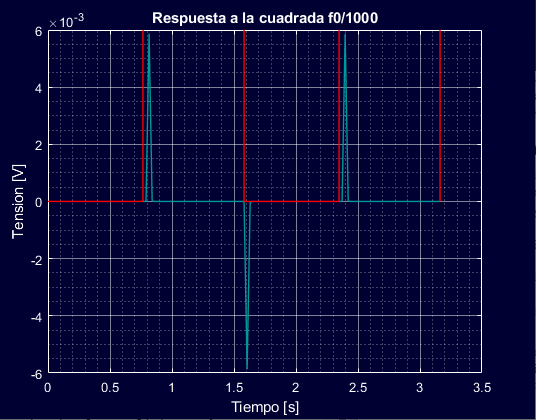
\includegraphics[scale = 0.9]{imagenes/respuesta_cuadrada_f0_1000.png}
     \centering
     \caption{Se'nal cuadrada de $\frac{f_0}{1000}$ en rojo (amplitud 1) , respuesta en turquesa}
    \end{figure}

    En este caso el semiperiodo de la se'nal cuadrada $\frac{T_{cuad}}{2} = 0.79s$ es mucho mayor que el tiempo de amortiguamiento $4\tau = 0.018s$ y por lo tanto si veremos a la respuesta amortiguarse dentro del semiperiodo. De hecho la relación entre $\frac{T_{cuad}}{2} y 4\tau$ nos puede indicar en que momento del semiperiodo se amortigua:
    
    \begin{center}
        $\frac{4\tau}{\frac{T_{cuad}}{2}} = 0.02$
    \end{center}
    
    Lo que significa que en aproximadamente un 2\% del tiempo en que la se'nal cuadrada esta en su valor máximo, la respuesta se amortigua. 

    \subsection{Respuesta a se'nales senoidales}
    Se excitará el filtro con tres se'nales senoidales de diferente frecuencia y se estudiará la respuesta del filtro a estas se'nales.
    Las frecuencias elegidas fueron: 
    \begin{itemize}
        \item $f_0 = \frac{w_0}{2\pi} = 632.47Hz$
        \item $f = \frac{314\frac{rad}{s}}{2\pi} = 50Hz$
        \item $f = \frac{100\frac{rad}{s}}{2\pi} = 15.91Hz$
    \end{itemize}

    \subsubsection{Respuesta a se'nal senoidal de $f_0 = \frac{w_0}{2\pi}$}
    
     \begin{figure}[!htb]
     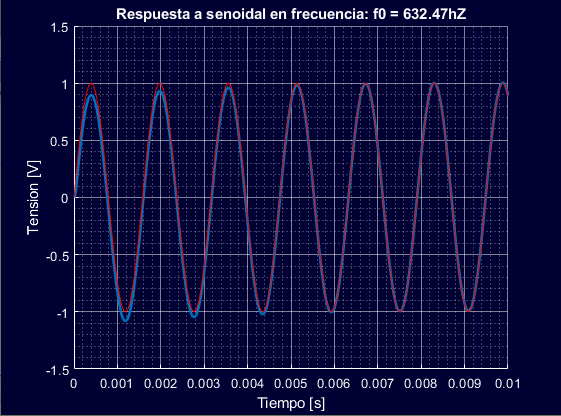
\includegraphics[scale = 0.9]{imagenes/senoidal_f0.png}
     \centering
     \caption{Respuesta a la senoidal de 632.47Hz en turquesa, se'nal senoidal en rojo}
    \end{figure}
    
    Observamos que tanto la se'nal de excitación, como la respuesta tienen y la misma amplitud y están en fase. Esto era previsible pues el diagrama de Bode de magnitud nos indicaba que la ganancia era unitaria para esta frecuencia ($w_0 = 3973.92\frac{rad}{s}$). Además el diagrama de Bode de fase nos indicaba que para esta frecuencia el desfase era de 0$\degree$
    
    \newpage
    
    \subsubsection{Respuesta a se'nal senoidal de $f = \frac{314\frac{rad}{s}}{2\pi} = 100Hz$}
    
    \begin{figure}[!htb]
    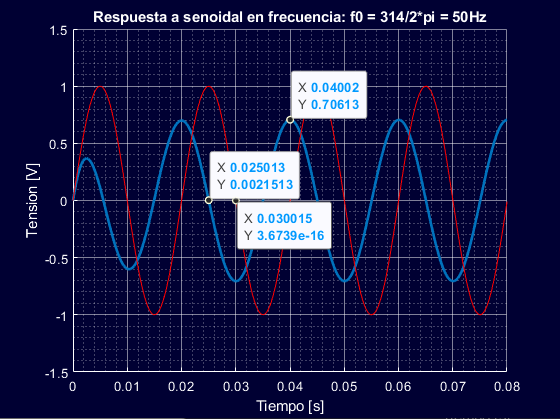
\includegraphics[scale = 0.9]{imagenes/senoidal_314_frecuencia_corte.png}
    \centering
    \caption{Respuesta a la senoidal de 50Hz en turquesa, se'nal senoidal en rojo}
    \end{figure}
    
    Recordemos que $314\frac{rad}{s}$ era una frecuencia para la cual la ganancia en magnitud era de -3dB, es decir de aproximadamente el 70\% . En el gráfico se puede ver que la amplitud máxima de la respuesta alcanza un valor de 0.70 como es esperado.  
    
    Respecto al desfase, según el diagrama de Bode de fase, se debería alcanzar un desfase de 90$\degree$. Para corroborar esto se marcaron dos puntos en la figura que nos permitirán calcular un desfase temporal $\Delta t$ entre las se'nales:
    
    \begin{center}
        $\Delta t = 0.03s - 0.0025s = 0.0005s$
    \end{center}
    
    A partir de esto, obtenemos el desfase en ángulos multiplicándolo por $w = 314\frac{rad}{s}$:
    
    \begin{center}
        $\Delta\phi = 314\frac{rad}{s} \Delta t = 1.57rad = \frac{\pi}{2}rad=90\degree$
    \end{center}
    
    \newpage
    
    \subsubsection{Respuesta a se'nal senoidal de $f = \frac{100\frac{rad}{s}}{2\pi} = 15.91Hz$}
    
    \begin{figure}[!htb]
    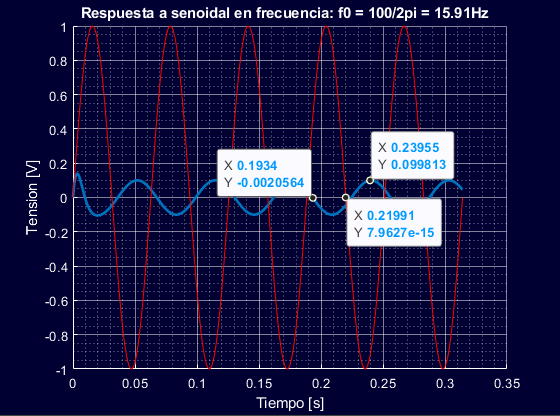
\includegraphics[scale = 0.9]{imagenes/senoidal_15.91Hz.png}
    \centering
    \caption{Respuesta a la senoidal de 15.91Hz en turquesa, se'nal senoidal en rojo}
    \end{figure}
    
    Se puede ver que la amplitud se redujo de 1V a 0.1V, es decir a un 10\% de la se'nal de entrada. Esto se corresponde con que a frecuencia $w = 100\frac{rad}{s}$ la ganancia en magnitud es de -20dB.
    
    Respecto del desfase podemos realizar el mismo procedimiento anterior con los puntos indicados en la figura:
    
     \begin{center}
        $\Delta t = 0.219s - 0.193s = 0.026s$\\
        $\Delta\phi = 100\frac{rad}{s} \Delta t = 2.6rad = 2.6rad\cdot\frac{180\degree}{\pi rad}= 148\degree$
    \end{center}
    
    Lo cual se corresponde con el diagrama de Bode de fase
    
    \newpage
    
    \section{Dise'no de filtro}
    
    En esta sección se explicara el proceso de dise'no de un filtro que tenga la función de transferencia H(s) deseada.
    
    \subsection{Cuestiones previas}
    Se desea dise'nar un filtro pasabanda con la función de transferencia:
    \begin{center}
        H(s) =$\frac{s^2 \cdot 2,527 \cdot 10^9}{s^4 + s^3 \cdot 7,153 \cdot 10^4 + s^2 \cdot 2,558 \cdot 10^9  +s \cdot 1,13\cdot 10^{12} +2,494 \cdot 10^{14} }$
    \end{center}
   Una forma de realizar esto es poniendo en cascada dos filtros: un pasabajos de segundo orden y pasaaltos de segundo orden cuyas transferencias tienen como forma general:
   \begin{center}
       $H(s)_{LP} = \frac{k_{LP}\cdot {w_{LP}}^2}{s^2 + s\cdot\frac{w_{LP}}{Q_{LP}} + {w_{LP}}^2}$\\
       $H(s)_{HP} = \frac{k_{HP}\cdot s^2}{s^2 + s\cdot\frac{w_{HP}}{Q_{HP}} + {w_{HP}}^2}$
   \end{center}
    Donde:
    \begin{itemize}
        \item $H(s)_{LP}$ es la transferencia del pasabajos
        \item $H(s)_{HP}$ es la transferencia del pasaaltos
        \item $w_{LP}$ y $w_{HP}$ son las frecuencias naturales de  los filtros
        \item $Q_{LP}$ y $Q_{HP}$ son los factores de calidad de los filtros
        \item $k_{LP}$ y $k_{HP}$ son los factores de ganancia de los filtros
    \end{itemize}
    
    Al colocar los filtros en cascada, la transferencia del filtro resultante es el producto de las transferencias de los filtros que la compononen:
    \begin{center}
        H(s) = $H(s)_{LP}\cdot H(s)_{HP} $
    \end{center}
    
    Para lograr construir el filtro pasabanda, necesitamos que la frecuencia $w_{HP}$ del pasaaltos sea menor a la frecuencia $w_{LP}$ del pasabajos. De esta forma habrá un rango de frecuencias que ambos filtros dejan pasar que conformaran el ancho de banda del pasabanda.
    Es por este motivo que asignaremos las siguientes frecuencias halladas en la sección 2.2.3:
    \begin{center}
        $w_{LP} = 50262.33\frac{rad}{s}$ \hspace{10mm}$w_{HP} = 314.19\frac{rad}{s}$
    \end{center}
    Los factores de calidad de estos filtros deben corresponderse, también, con los hallados en la sección 2.2.3:
     \begin{center}
        $Q_{LP} = 0.7$ \hspace{10mm}$Q_{HP} = 0.7$
    \end{center}
    Observando el diagrama de Bode pudimos observar que para el rango de frecuencias en el ancho de banda del circuito, la ganancia en tensión era unitaria o de 0dB. Esto lo podemos lograr si los factores de ganancia en tensión de los filtros pasabajos y pasaaltos son unitarios:
    \begin{center}
        $K_{LP} = 1$ \hspace{10mm}$K_{HP} = 1$
    \end{center}
    
 
    Por ultimo debemos escoger los filtros pasabajos y pasaltos que usaremos para construir nuestro filtro pasabanda. Se eligieron los filtros pasaaltos y pasabajos de Sallen-Key expuestos en la siguiente secci'on.
    
    \subsection{Filtros de Sallen-Key}
    
    \subsubsection{Filtro pasabajos de Sallen Key}
    El filtro pasabajos de Sallen-Key consta de cuatro resistores y dos capacitores dispuestos como indica la siguiente figura:
    
    \vspace{2mm}
    \begin{figure}[!htb]
    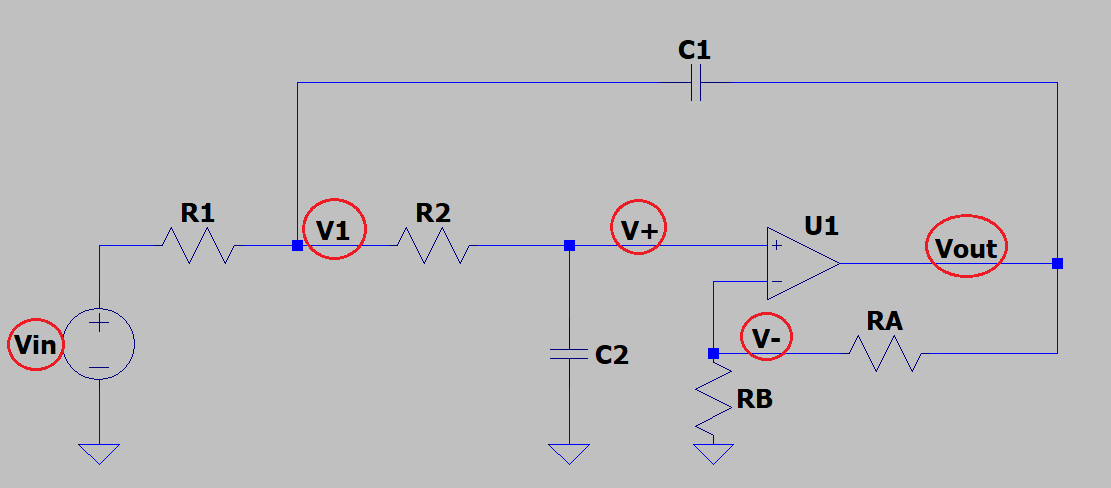
\includegraphics[scale = 0.5]{imagenes/FiltroPasabajosDeSallenKey.png}
    \centering
    \caption{Filtro pasabajos de Sallen-Key}
    \end{figure}
    
    Realizaremos la deducción de la transferencia para este filtro a partir del método de nodos. Planteamos las ecuaciones de nodos para los nodos $V_{1}$, $V_{+}$ y $V_{-}$ (Observación: reemplazamos $V_{in}$ por 1 y buscamos $V_{out}$):
    \begin{itemize}
        \item $V_1:$ \hspace{5mm}$0 = V_1(\frac{1}{R_1}+\frac{1}{R_2}+sC_1)-V_{+}(\frac{1}{R_2})-1(\frac{1}{R_1})-V_{out}(sC_1)$
        \item $V_{+}:$ \hspace{5mm} $0 = V_{+}(\frac{1}{R_2}+sC_2) - V_1(\frac{1}{R_2})$
        \item $V_{-}:$ \hspace{5mm} $0 = V_{-}(\frac{1}{R_A}+\frac{1}{R_B})-V_{out}(\frac{1}{R_A})$
    \end{itemize}
        
    Buscaremos despejar de la ecuación de nodo de $V_{+}$ a $V_{1}$ y de la ecuacion de nodo de $V_{-}$ a $V_{-}$. Llamaremos V a $V_{-} = V_{+} = V$
    \begin{itemize}
        \item De la ecuación de $V_+$:\hspace{5mm} $V_1 = V(1+s R_2 C_2)$
        \item De la ecuación de $V_-$: \hspace{5mm} $V = V_{out}(\frac{R_B}{R_B + R_A}) $
    \end{itemize}
    Reescribiendo estas dos ecuaciones en función de $V_{out}$ y reemplazando $\frac{R_B}{R_B + R_A}$ por $\frac{1}{k}$ (y por lo tanto $k = 1+\frac{R_A}{R_B}$) llegamos a las siguientes ecuaciones:
    \begin{itemize}
        \item $V_1 = V_{out}\frac{1}{k}(1+sR_2C_2)$
        \item $V = V_{out}\frac{1}{k}$
    \end{itemize}
    
    
    Multiplicamos la ecuación de nodo correspondiente a $V_{1}$ por $R_1R_2$ y luego reemplazamos por las expresiones halladas anteriormente para V y $V_1$ en función de $V_out$
    \begin{itemize}
        \item ec $V_1\cdot R_1 R_2:$\hspace{5mm} $0=V_1(R_2+R_1+R_1R_2C_1s)-V(R_1)-R_2-V_{out}(sC_1R_1R_2)$
        \item $0 = V_{out}\frac{1}{k}(1+sR_2C_2)(R_2+R_1+R_1R_2C_1s) -V_{out}\frac{1}{k}(R_1)-R_2-V_{out}(sC_1R_1R_2)$
        \item $R_2 = V_{out}(\frac{1}{k}(1+R_2C_2s)(R_2+R_1+R_1R_2C_1s-R_1)-sC_1R_1R_2)$
        \item $R_2 = V_{out}(\frac{1}{k}(R_2+R_1R_2C_1s+R_2^2C_2s+R_1R_2C_2s+R_2^2R_1C_1C_2s^2)-sC_1R_1R_2$
        \item $k = V_{out}(1+R_1C_1s+R_2C_2s+R_1C_2s+R_2R_1C_1C_2s^2 - ksC_1R_1)$
        \item $k = V_{out}(1+s(R_1C_1+R_2C_2+R_1C_2-kR_1C_1) + R_1R_2C_1C_2s^2 )$
        \item $k = V_{out}(1+s[R_1C_1(1-k)+(R_2+R_1)C_2] + R_1R_2C_1C_2s^2 )$
        \item $V_{out} = \frac{k (\frac{1}{R_1R_2C_1C_2})}{s^2 + s(\frac{1-k}{R_2C_2}+\frac{1}{(R_1//R_2)C_1})+ \frac{1}{ R_1R_2C_1C_2}}$
    \end{itemize}
    
    De manera que la transferencia para el filtro pasabajos de Sallen-Key resulta:
    \begin{center}
        H(s) = $\frac{k (\frac{1}{R_1R_2C_1C_2})}{s^2 + s(\frac{1-k}{R_2C_2}+\frac{1}{(R_1//R_2)C_1})+ \frac{1}{ R_1R_2C_1C_2}}$
    \end{center}
    
    Donde podemos observar que:
    \begin{itemize}
        \item $w_{LP}^2$ = $\frac{1}{R_1R_2 C_1 C_2}$
        \item $k_{LP}$ = $1+\frac{R_A}{R_B}$
    \end{itemize}
    
    Observamos que para el caso en que el factor de ganancia del filtro sea $K_{LP} = 1$ se cumple que:
    \begin{center}
    $H(s)_{LP}$ = $\frac{(\frac{1}{R_1R_2C_1C_2})}{s^2 + s(\frac{1}{(R_1//R_2)C_1})+ \frac{1}{ R_1R_2C_1C_2}}$\\
    \vspace{4mm}
    $1 = 1+\frac{R_A}{R_B} \Rightarrow \frac{R_A}{R_B} = 0 \Rightarrow R_A = 0$
    \end{center}
    
    Observamos también que de esta manera el valor de $R_B$ deja de ser relevante y por lo tanto podremos removerlo del circuito. En la siguiente figura mostramos una forma general del circuito pasabajos de Sallen-Key de ganancia unitaria que utilizaremos para el dise'no de nuestro filtro pasabanda:
    
     \begin{figure}[!htb]
    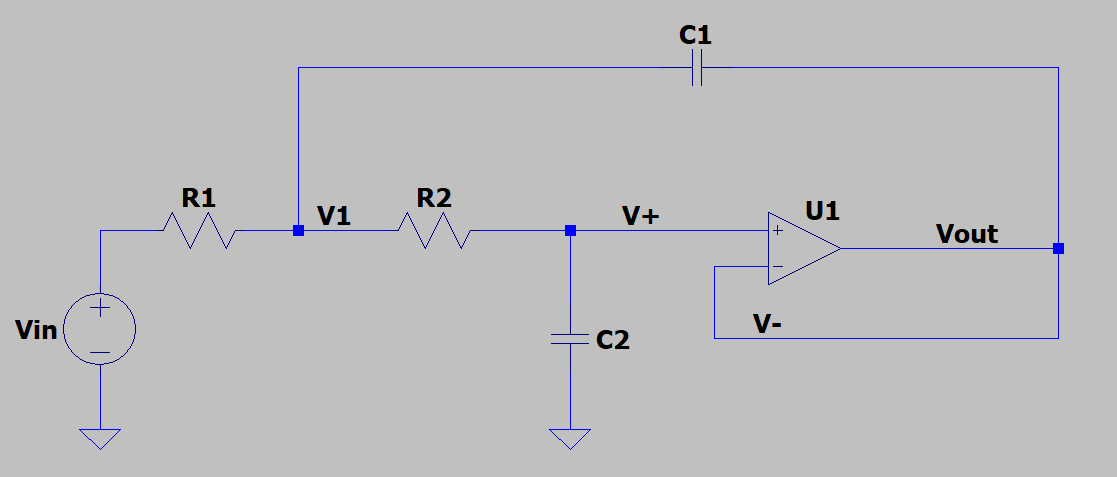
\includegraphics[scale = 0.5]{imagenes/FiltroPasabajosDeSallenKeyGananciaUnitaria.png}
    \centering
    \caption{Filtro pasabajos de Sallen-Key de ganancia unitaria}
    \end{figure}
    
    \newpage
    
    \subsubsection{Filtro pasaaltos de Sallen-Key}
    El filtro pasaaltos de Sallen-Key es similar al filtro pasabajos. La diferencia entre estos filtros es que se intercambian las posiciones de la resistencias R1 y R2 por las de los capacitores C1 y C2 respectivamente obteniendo el siguiente circuito:
    \vspace{2mm}
    \begin{figure}[!htb]
    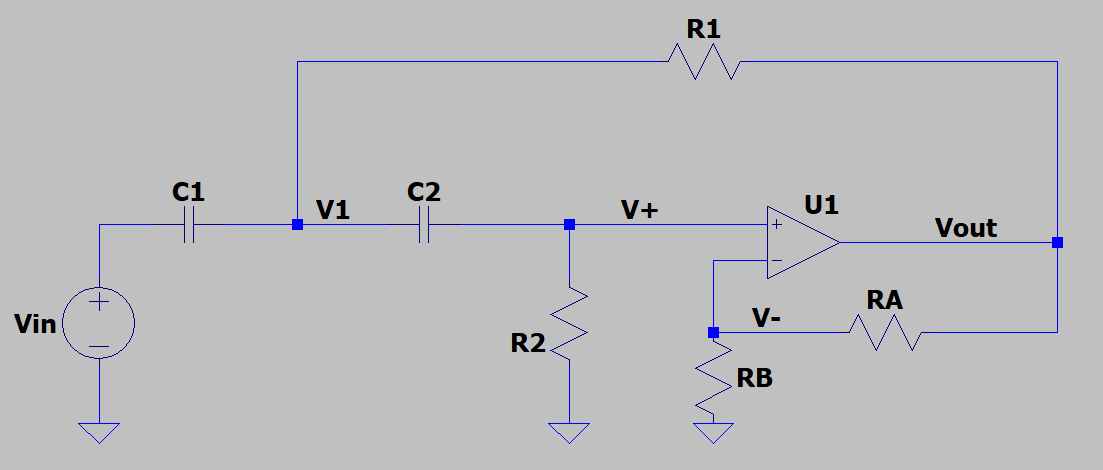
\includegraphics[scale = 0.5]{imagenes/FiltroPasaaltosDeSallenKey.jpg}
    \centering
    \caption{Filtro pasaaltos de Sallen-Key}
    \end{figure}
    
    En particular, nos interesa estudiar el caso para el que la ganancia es unitaria: 
    \vspace{2mm}
    \begin{figure}[!htb]
    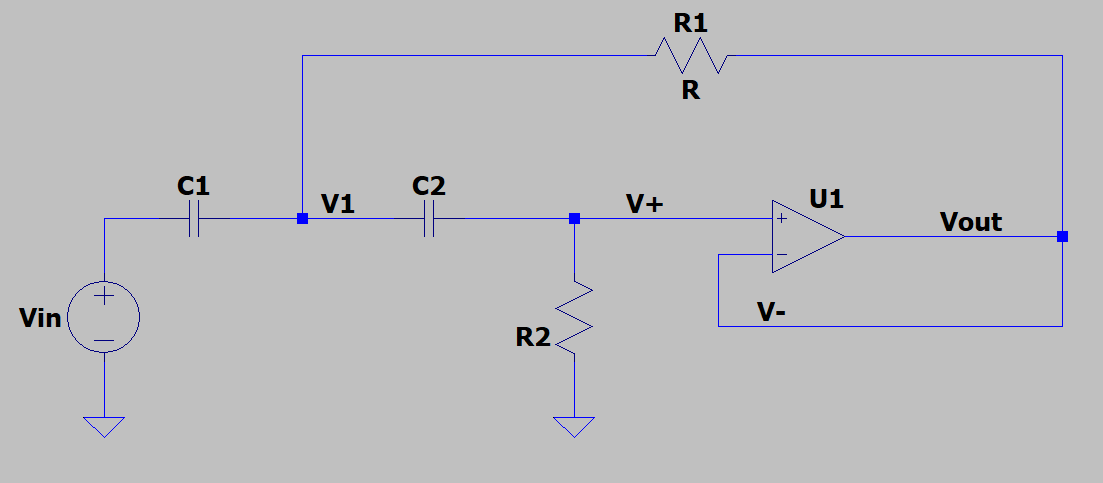
\includegraphics[scale = 0.5]{imagenes/FiltroPasaaltosDeSallenKeyDeGananciaUnitaria.png}
    \centering
    \caption{Filtro pasaaltos de Sallen-Key de ganancia unitaria}
    \end{figure}
    
    Podemos obtener la transferencia de esta filtro a partir de la transferencia del filtro pasabajos de Sallen-Key de ganancia unitaria. Debemos reemplazar las admitancias de $R_1$ y $R_2$ por las de $C_1$ y $C_2$ y viceversa, es decir:
    
   \begin{itemize}
       \item $\frac{1}{R_1} = sC_1 \Rightarrow R_1 = \frac{1}{sC_1}$
       \item $\frac{1}{R_2} = sC_2 \Rightarrow R_2 = \frac{1}{sC_2}$
       \item $sC_1 = \frac{1}{R_1} \Rightarrow C_1 = \frac{1}{sR_1}$
       \item $sC_2 = \frac{1}{R_2}  \Rightarrow C_2 = \frac{1}{sR_2}$
   \end{itemize}
    
    Realizando estos cambios en la transferencia del pasabajos obtenemos:

    \begin{center}
         \item $H(s)_{HP} = \frac{s^4 C_1C_2R_1R_2}{s^2+s^3(C_1+C_2)R_1+s^4C_1C_2R_1R_2}$
    \end{center}
   
    Y simplificando esta expresión hallamos la transferencia del filtro pasaaltos de Sallen-Key de ganancia unitaria que utilizaremos en nuestro dise'no:
    \begin{center}
        $H(s)_{HP}= \frac{s^2}{s^2+s\frac{1}{R_2(C_1//C_2)}+\frac{1}{R_1R_2C_1C_2}}$
    \end{center}
    
    \subsubsection{Justificación de la elección de los filtros de Sallen-Key}
    El motivo por el cual se escogieron los filtros de ganancia unitaria de Sallen-Key es que utilizan una cantidad razonable de resistores y capacitores (dos de cada uno) logrando armar un filtro resultante con pocos recursos.
    Adem'as particularmente en el caso del filtro pasaaltos, escogiendo los valores deseados para $w_0$, Q y los capacitores, los valores de las resistencias quedan completamente determinados por lo que el dise'no del filtro se vuelve simple. 
    
    \subsection{Valores normalizados de los componentes}
    Una vez definidos los filtros pasaaltos y pasabajos que utilizaremos y sus transferencias, debemos escoger los valores normalizados de resistencias y capacitores que nos permitan filtrar las frecuencias deseadas.
    
    Se definieron primero los valores de los capacitores y luego los de los resistores. Se utilizaron valores normalizados de la serie del 10\% tanto para los capacitores como para los resistores. 
    Ademas los valores de los capacitores se encuentran en el rango [1nF, 1µF] y los resistores en el rango [1kΩ, 1MΩ].

    \subsubsection{Valores normalizados del filtro pasaaltos}
    Debemos dise'nar un filtro pasaaltos se Sallen-Key de ganancia unitaria que cumpla:
    \begin{center}
        $w_{0} = 314.19\frac{rad}{s} \hspace{5mm} Q = 0.7$
    \end{center}
    
    
    Recordando que la transferencia para el filtro era: 
     \begin{center}
        $H(s)_{HP}= \frac{s^2}{s^2+s\frac{1}{R_2(C_1//C_2)}+\frac{1}{R_1R_2C_1C_2}}$
    \end{center}
    
    Observamos que:
    \begin{center}
        (a) ${w_0}^2 = \frac{1}{R_1R_2C_1C_2}$\\
        (b) $\frac{w_0}{Q} = \frac{1}{R_2(C_1//C_2)}$
    \end{center}
    Despejando $R_2$ de la ecuación (b) y $R_1$ de la ecuación (a) obtenemos:
    \begin{center}
        $R_2= \frac{Q}{w_0 \cdot (C_1//C_2)}$\\
        $R_1= \frac{1}{w_0 \cdot Q \cdot (C1+C2)}$
    \end{center}
    Por lo que logramos escribir a los resistores en función de los capacitores, de $w_0$ y de $Q$. Esto nos da libertad para escoger los valores de $C_1$ y $C_2$ de manera independiente hasta lograr que los valores de $R_1$ y $R_2$ se encuentren en la serie del 10\%. Escogiendo $C_2$ = 12nF y $C_1$= 68nF obtuvimos los siguientes valores para $R_1$ y $R_2$:
    
    \begin{center}
        $R_1 =  56.835k\Omega$ \hspace{5mm} $R_2 = 218.43k\Omega$
    \end{center}
    
    Que aproximaremos a los siguientes valores normalizados:
    \begin{center}
        $R_1 = 56k\Omega$ \hspace{5mm} $R_2 = 220k\Omega$
    \end{center}
    
    De manera que la transferencia para el filtro pasaaltos resulta:
    \begin{center}
        $H(s)_{HP} = \frac{s^2}{s^2 +s\cdot448.83 + 99461.4}$
    \end{center}

    Mostramos el diagrama de Bode para este filtro. Observamos que logramos que a frecuencia $w_0 = 314\frac{rad}{s}$ la ganancia en magnitud sea de aproximadamente -3dB como deseábamos.
  
    \begin{figure}[!htb]
    \includegraphics[scale = 1]{imagenes/BodePasaaltos.png}
    \centering
    \caption{Diagrama de Bode - Pasaaltos de Sallen-Key}
    \end{figure}
  
    \subsubsection{Valores normalizados filtro pasabajos}
    Para el filtro pasabajos debíamos dise'narlo de manera que tenga ganancia unitaria y:
    \begin{center}
        $w_0 = 50262.33\frac{rad}{s} \hspace{5mm} Q = 0.7$
    \end{center}
    Recordemos que la función de transferencia para el filtro pasabajo de ganancia unitaria de Sallen-Key era: 
    \begin{center}
        $H(s)_{LP}$ = $\frac{(\frac{1}{R_1R_2C_1C_2})}{s^2 + s(\frac{1}{(R_1//R_2)C_1})+ \frac{1}{ R_1R_2C_1C_2}}$
    \end{center}
    Donde:\begin{center}
        (a) ${w_0}^2 = \frac{1}{R_1R_2C_1C_2}$\\
      (b) $\frac{w_0}{Q} = \frac{1}{C_1(R_1//R_2)}$
    \end{center}
     
     Despejando $R_1//R_2$ de la ecuación (b) y $C_2$ de la primera ecuación:
     \begin{center}
         $R_1//R_2 = \frac{Q}{w_0C_1}$
         $C_2=\frac{1}{{w_0}^2 R_1  R_2  C_1}$
     \end{center}
     
     Lo primero que hacemos es elegir $C_1$ arbitrariamente:
     
    \begin{center}
        $C_1 = 4.7nF$
    \end{center}
    
    Esto determina que $R_1//R_2$ debe ser: 
    
    \begin{center}
             $R_1//R_2 = 2.9632k\Omega$
    \end{center}
   
   De manera que resta seleccionar $R_1$ y $R_2$ de manera de cumplir lo anterior y que el capacitor $C_2$ sea aproximadamente un valor normalizado. Se escogieron:
\begin{center}
    $R_1 = 4.7k\Omega$ \hspace{5mm} $R_2 = 8.2k\Omega$ \hspace{2mm}$\Rightarrow \hspace{2mm}  R_1//R_2 = 2.9876k\Omega$ y $C_2 = 2.1853nF$
\end{center}

    Por lo que escogemos un $C_2$ de:
    
    \begin{center}
        $C_2 = 2.2nF$
    \end{center}
     
     Con estos valores la transferencia del pasabajo resulta:
     
     \begin{center}
     $H(s)_{LP} = \frac{2.51\cdot10^9}{s^2+ 7.12\cdot10^4 + 2.51\cdot10^9}$    
     \end{center}
     
    Mostramos el diagrama de Bode para este filtro.
    Podemos ver que para frecuencia aproximadamente $50262.33\frac{rad}{s}$ la ganancia es de -3dB como deseábamos: 
     
    \begin{figure}[!htb]
    \includegraphics[scale = 1]{imagenes/BodePasabajos.png}
    \centering
    \caption{Diagrama de Bode - Pasabajos de Sallen-Key}
    \end{figure}
  
  \newpage
  
    \subsection{Análisis del filtro dise'nado}
    Como dijimos para construir el pasabanda debemos poner los filtros pasaalto y pasabajos conseguidos anteriormente en cascada resultando:
    
     \begin{figure}[!htb]
    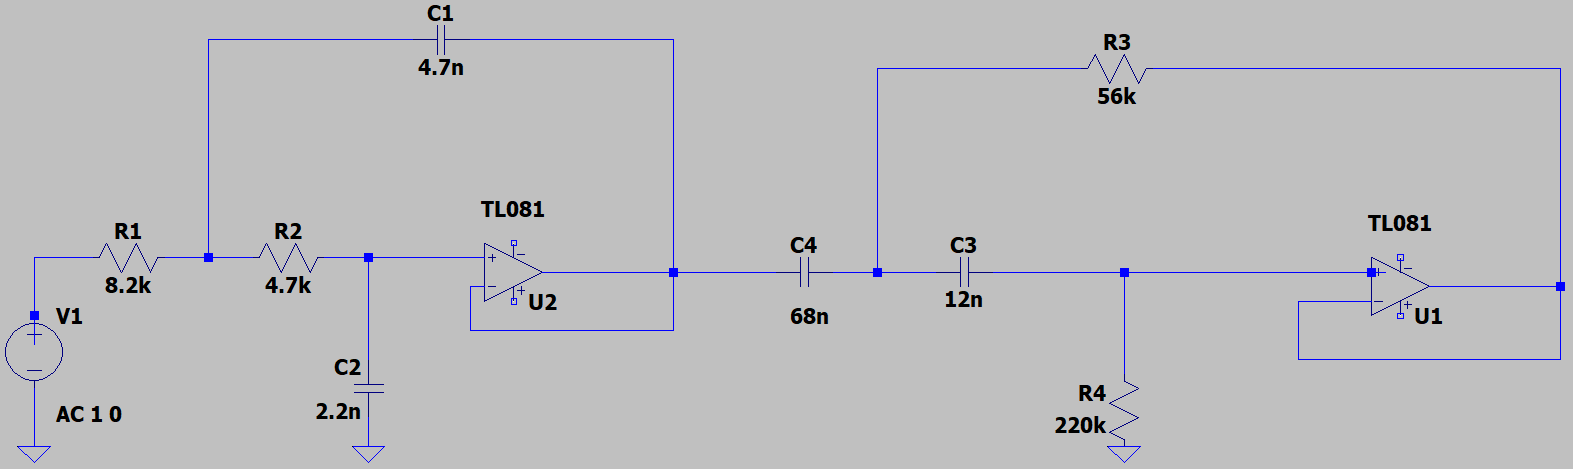
\includegraphics[scale = 0.40]{imagenes/FiltroCascada.png}
    \centering
    \caption{Filtro pasabanda de cuarto orden dise'nado}
    \end{figure}
    
    \subsubsection{Transferencia}
    
    Su función de transferencia la conseguimos multiplicando $H(s)_{LP}\cdot H(s)_{HP}$:
    \begin{center}
          H(s) = $\frac{2.51 \cdot 10^9 s^2}{s^4 + 7.165 \cdot10^4 s^3 + 2.542 \cdot 10^9 s^2 + 1.134 \cdot 10^{12} s + 2.496 \cdot 10^{14}}$
    \end{center}
    
    La cual es muy similar a la ideal: 
   \begin{center}
       H(s) = $
    \frac{s^2 \cdot 2,527 \cdot 10^9}
    {s^4 + s^3 \cdot 7,153 \cdot 10^4 + 
     s^2 \cdot 2,558 \cdot 10^9  +
     s \cdot 1,13\cdot 10^{12} +
     2,494 \cdot 10^{14} }
$
   \end{center}
   
   \subsubsection{P'arametros del filtro}
   Mostramos los valores de las frecuencias $w_a$ y $w_b$ ideales y obtenidos. Lo mismo para los valores de $Q_a$ y $Q_b$:
   \begin{center}
        \begin{tabular}{| c | c | c | c |}
        \hline
        Parametro & Ideal & Obtenido  & Error\\ \hline
        $w_a$ & 50262.33& 50093.78& 0.33\% \\
        $w_b$ &  314.19& 315.39& 0.2\%\\
        $Q_a$ &  0.70& 0.703& 0.42\% \\
        $Q_b$ & 0.70&0. 704& 0.57\%\\ \hline
        \end{tabular}
   \end{center}

   
   
   Las diferencias se deben a que el filtro dise'nado está construido a partir de valores normalizados de resistencias y capacitores por lo que no podemos construir un filtro que sea exactamente igual al dado.
   
   Sin embargo las siguientes simulaciones nos muestran que el filtro dise'nado con valores normalizados comparte las mismas características que el ideal.
   
   \newpage
   
   \subsubsection{Diagrama de Bode}
   
   Mostramos el diagrama de Bode obtenido en Matlab para esta transferencia: 
   \begin{figure}[!htb]
    \includegraphics[scale = 0.90]{imagenes/BodeMatlabMiFiltro.png}
    \centering
    \caption{Diagrama de bode del filtro pasabanda de cuarto orden dise'nado}
    \end{figure}
    
    El cual es muy similar al obtenido en la sección 2.3
    
    Además se muestra la respuesta en frecuencia obtenida para el filtro dise'nado en LTSpice:
    \begin{figure}[!htb]
    \includegraphics[scale = 0.7]{imagenes/bode_Spice.png}
    \centering
    \caption{Diagrama de Bode del filtro pasabanda de cuarto orden dise'nado obtenida en LTSpice}
    \end{figure}
    
    Hay que observar que LTSpice muestra el eje de frecuencias en f = $\frac{w}{2\pi}$ [Hz] mientras que Matlab lo muestra en $w$ $[\frac{rad}{s}]$. Es por estee motivo que los -3dB de ganancia se encuentran en las frecuencias indicadas en el gráfico: f = 50Hz $(314\frac{rad}{s})$ y f = 8000Hz $(50265\frac{rad}{s})$
    
    \newpage
    
    \subsubsection{Respuesta al impulso}
  
    Mostramos en rojo la respuesta al impulso obtenida para el filtro  dise'nado y en turquesa la respuesta al impulso obtenida en la sección 2.5
  
   \begin{figure}[!htb]
    \includegraphics[scale = 0.9]{imagenes/comparacion_impulso_miFiltro_impulse.png}
    \centering
    \caption{Respuesta al impulso del filtro dise'nado en rojo, respuesta al impulso hallada en la sección 2.5 en turquesa}
    \end{figure}
    \vspace{2mm}
    Podemos ver -tanto para esta respuesta como para las que siguen- que la respuesta del filtro dise'nado se superpone con la respuesta que otorga Matlab con su funcion impulse() y que fue analizada en la secci'on 2.5. 
    
    \vspace{6mm}
    
    Esto nos indica que a pesar de que el filtro dise'nado no tiene exactamente la misma transferencia que la dada (porque fue construido con resistencias y capacitores a valores normalizados), son lo suficientemente similares como para tener las mismas respuestas. 
    
    \vspace{6mm}
    
    Procederemos a mostrar las respuestas a las misma se'nales obtenidas en las secciones anteriores y a compararlas con la otorgada por Matlab para la transferencia ideal y con la otorgada por Spice
    
    \newpage
    
    
    \subsubsection{Respuesta al escalón}
    
    Se muestra la respuesta al escalón hallada en la sección 2.4 en turquesa y la respuesta al escalón hallada para el filtro dise'nado en rojo:
    
    \begin{figure}[!htb]
    \includegraphics[scale = 0.9]{imagenes/comparacion_escalon_miFiltro_step.png}
    \centering
    \caption{Respuesta al escalón del filtro dise'nado en rojo, respuesta al escalón hallada en la seccion 2.4 en turquesa, respuesta de LTSpice en verde}
    \end{figure}
    
    Se muestra ahora la respuesta al escalón para el filtro dise'nado en LTSpice:
    \begin{figure}[!htb]
    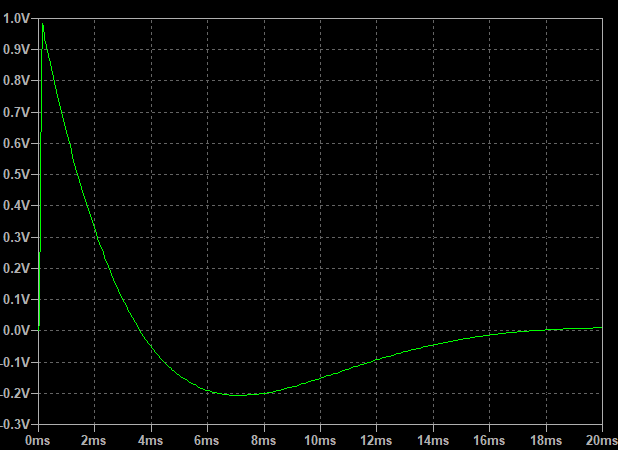
\includegraphics[scale = 0.8]{imagenes/escalon_Spice.png}
    \centering
    \caption{Respuesta al escalón en LTSpice del filtro dise'nado}
    \end{figure}
    
    
    \subsubsection{Respuesta a se'nales cuadradas}
    
    Se muestran comparaciones entre las respuestas halladas en la sección 2.7 y las respuesta del filtro dise'nado. Adem'as se muestra la respuesta que genera LTSpice:
    
    \begin{figure}[!htb]
    \includegraphics[scale = 0.9]{imagenes/comparacion_cuadrada_f0.png}
    \centering
    \caption{Respuesta a la cuadrada de $f_0 = 632.47Hz$ del filtro dise'nado en rojo, respuesta a la cuadrada hallada en la sección 2.7 en turquesa, respuesta de LTSpice en verde}
    \end{figure}
    
    \begin{figure}[!htb]
    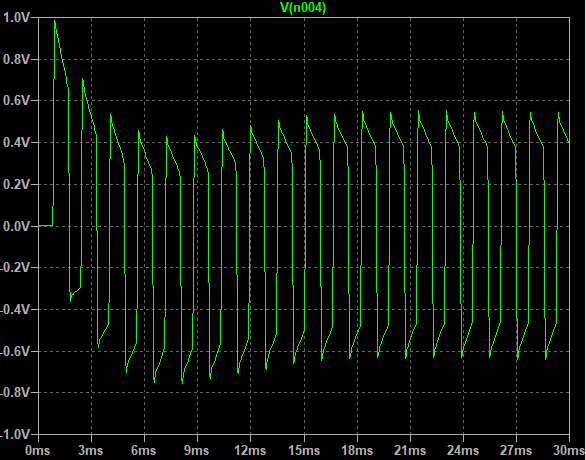
\includegraphics[scale = 0.8]{imagenes/cuadrada_f0_Spice.png}
    \centering
    \caption{Respuesta a la cuadrada de $f_0 = 632.47Hz$ en LTSpice del filtro dise'nado}
    \end{figure}
    
    \newpage
    
    \begin{figure}[!htb]
    \includegraphics[scale = 0.9]{imagenes/comparacion_cuadrada_10f0.png}
    \centering
    \caption{Respuesta a la cuadrada de $10f_0 = 6324.7Hz$ del filtro dise'nado en rojo, respuesta a la cuadrada hallada en la sección 2.7 en turquesa, respuesta de LTSpice en verde}
    \end{figure}
    
    \begin{figure}[!htb]
    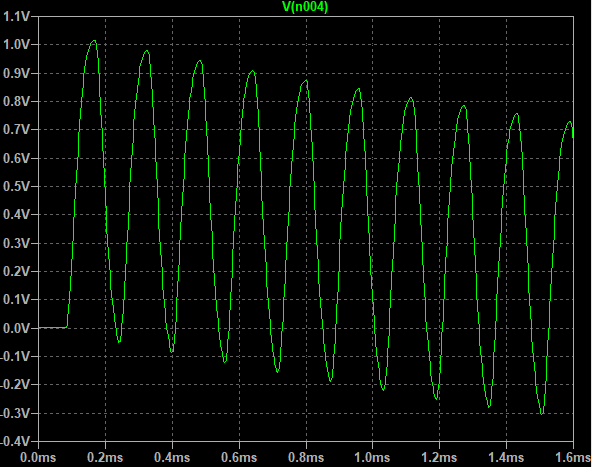
\includegraphics[scale = 0.83]{imagenes/cuadrada_10f0_Spice.png}
    \centering
    \caption{Respuesta a la de $10f_0 = 6324.7Hz$ cuadrada en LTSpice del filtro dise'nado}
    \end{figure}
    
    \newpage
    
    \begin{figure}[!htb]
    \includegraphics[scale = 0.9]{imagenes/comparacion_cuadrada_f0_10.png}
    \centering
    \caption{Respuesta a la cuadrada de $\frac{f_0}{10} = 63.247Hz$  del filtro dise'nado en rojo, respuesta a la cuadrada hallada en la sección 2.7 en turquesa, respuesta de LTSpice en verde}
    \end{figure}
    
    \begin{figure}[!htb]
    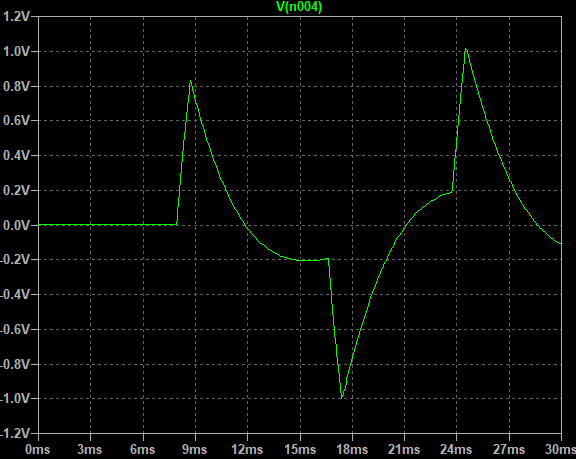
\includegraphics[scale = 0.83]{imagenes/cuadrada_f0_10_Spice.png}
    \centering
    \caption{Respuesta a la cuadrada de $\frac{f_0}{10} = 63.247Hz$ en LTSpice del filtro dise'nadoo}
    \end{figure}
    
    \newpage
    
    \subsubsection{Respuesta a se'nales senoidales}
    Se muestran comparaciones entre las respuestas a se'nales senoidales halladas en la sección 2.8 y las respuestas del filtro dise'nado. Adem'as se muestra la respuesta que genera LTSpice:
    
    \begin{figure}[!htb]
    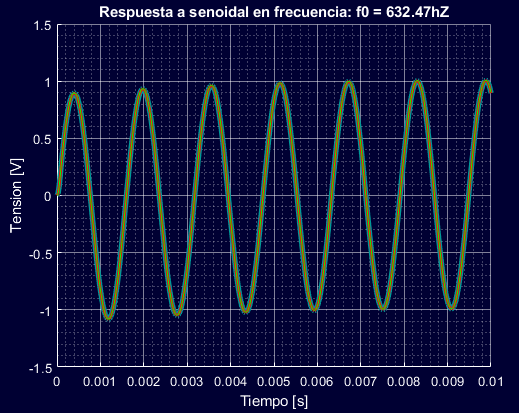
\includegraphics[scale = 0.9]{imagenes/comparacion_senoidal_632.47Hz.png}
    \centering
    \caption{Respuesta a la senoidal de $f_0 = 632.47Hz$ del filtro dise'nado en rojo, respuesta a la cuadrada hallada en la sección 2.7 en turquesa, respuesta de LTSpice en verde}
    \end{figure}
    
    \begin{figure}[!htb]
    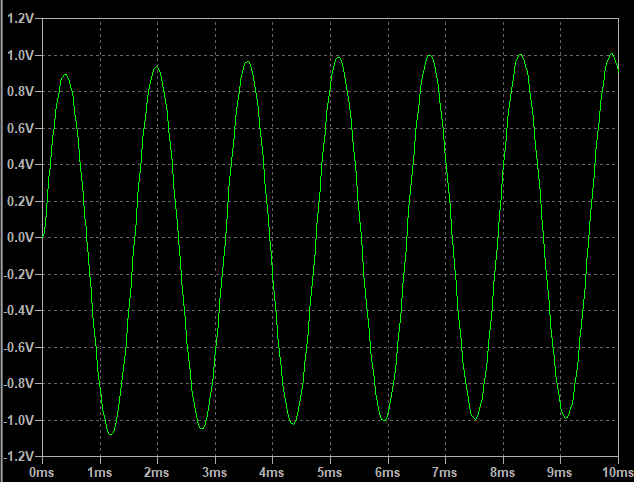
\includegraphics[scale = 0.75]{imagenes/senoidal_f0_Spice.png}
    \centering
    \caption{Respuesta a la senoidal de $f_0 = 632.47Hz$ en LTSpice del filtro dise'nado}
    \end{figure}
    
    \newpage
    
    \begin{figure}[!htb]
    \includegraphics[scale = 0.9]{imagenes/comparacion_senoidal_50Hz.png}
    \centering
    \caption{Respuesta a la senoidal de $f = 50Hz$ del filtro dise'nado en rojo, respuesta a la cuadrada hallada en la sección 2.7 en turquesa, respuesta de LTSpice en verde}
    \end{figure}
    
    \begin{figure}[!htb]
    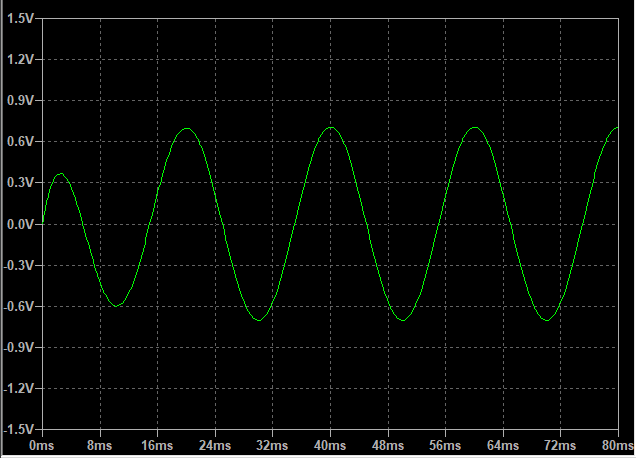
\includegraphics[scale = 0.83]{imagenes/senoidal_50Hz_Spice.png}
    \centering
    \caption{Respuesta a la senoidal de $f = 50Hz$ cuadrada en LTSpice del filtro dise'nado}
    \end{figure}
    
    \newpage
    
    \begin{figure}[!htb]
    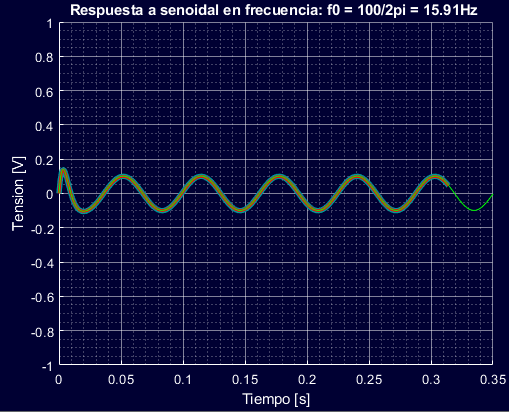
\includegraphics[scale = 0.9]{imagenes/comparacion_senoidal_15Hz.png}
    \centering
    \caption{Respuesta a la senoidal de $f = 15Hz$  del filtro dise'nado en rojo, respuesta a la cuadrada hallada en la sección 2.7 en turquesa, respuesta de LTSpice en verde}
    \end{figure}
    
    \begin{figure}[!htb]
    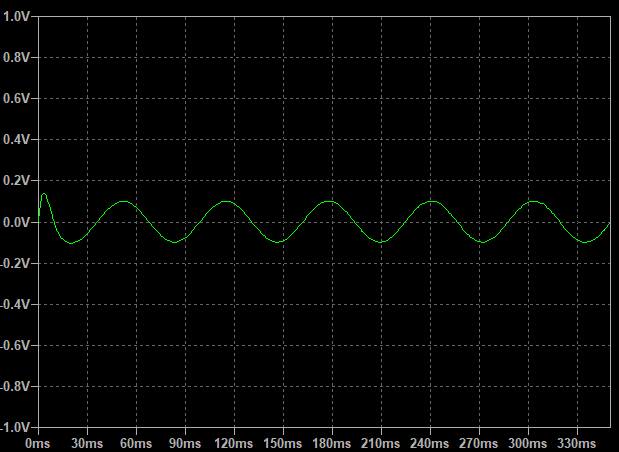
\includegraphics[scale = 0.83]{imagenes/senoidal_15.91Hz_Spice.png}
    \centering
    \caption{Respuesta a la cuadrada de $f = 15Hz$ en LTSpice del filtro dise'nado}
    \end{figure}
    
    \newpage
    
    \section{Cálculo an'alitco de las respuestas}
    
    En esta secci'on se deucir'an las respuestas al impulso, al escal'on y a la se'nal senoidal de 50Hz de manera an'alitica.
    
    A partir de la transferencia es posible obtener la respuesta en el campo de frecuencias complejas $V_{out}(s)$:  
    \begin{center}
        $H(s) = \frac{V_{out}(s)}{V_{in}(s)}$\\
        $V_{out}(s) = H(s)\cdot V_{in}(s)$
    \end{center}

    Por lo tanto, conociendo la transformada inversa de Laplace del producto de la tensi'on de entrada $V_{in}(s)$ con la transferencia H(s) podemos encontrar la respuesta temporal $V_{out}(t)$ a una tensión de entrada $V_{in}(t)$. Es decir: 
    
    \begin{center}
        $V_{out}(t)$ = $L^{-1}[V_{out(s)}]$ =$L^{-1}[H(s)\cdot V_{in}(s)] $
    \end{center}
    
    \subsection{Respuesta al impulso}
    
    Para hallar la respuesta al impulso o a la delta debemos identificar $V_{in}(t)$ y $V_{in}(s)$:
    \begin{center}
        $V_{in}(t) = \delta(t) \hspace{2mm} \Rightarrow  \hspace{2mm} V_{in}(s) = 1$
    \end{center}
    
    Por lo tanto para hallar la respuesta al impulso debemos antitransformar la transferencia H(s) pues:
    \begin{center}
        $V_{out}(t) = L^{-1}[H(s) \cdot V_{in}(s)] = L^{-1}[H(s)]$
    \end{center}
  
    Con este propósito, factorizamos el denominador de la transferencia en dos polinomios a coeficientes reales de segundo grado obteniendo:
    
    \begin{center}
        $H(s) = \frac{s^2 \cdot 2,527 \cdot 10^9}{(s^2+ s \cdot 444.5 + 98714.54)(s^2 +s \cdot 7.11\cdot 10^{4} + 2.53\cdot10^{9})} $
    \end{center}
    
    Procedemos a buscar una descomposición en fracciones simples del tipo:
    
    \begin{center}
          $H(s) = \frac{A s + B}{(s^2+ s \cdot 444.5 + 98714.54)} +  \frac{Cs + D}{(s^2 +s \cdot 7.11\cdot 10^{4} + 2.53\cdot10^{9})}$
    \end{center}
    
    Donde las constantes A, B, C y D deben ser tal que:
    
    \begin{center}
        $(As+B)(s^2 +s \cdot 7.11\cdot 10^{4} + 2.53\cdot10^{9})+(Cs+D)(s^2+ s \cdot 444.5 + 98714.54) = s^2 \cdot 2,527 \cdot 10^9$
    \end{center}
    
    Utilizando la notación eN para expresar $10^N$ podemos reescribir el miembro izquierdo como:
    
    \begin{center}
        \footnotesize$(A+C)s^3+(A7.11e4 +B+C444.5+D)s^2+(A2.53e9 + B7.11e4+ C98714.54 +D444.5)s+ (B2.53e9 + D98714.54)$
    \end{center}
    
    Por lo que restar resolver el siguiente sistema de ecuaciones lineales para hallar las constantes A,B,C y D:
    \begin{center}
    $A+C = 0$\\
    $A7.11e4 +B+C444.5+D = 2.527e9$\\
    $A2.53e9 + B7.11e4+ C98714.54 +D444.5 = 0$\\
    $B2.53e9 + D98714.54 = 0$
    \end{center}
    
    Con resultados:
    \begin{center}
        $A=-447,8 \hspace{5mm}
        B=-9,984\cdot10^4 \hspace{5mm}
        C=447,8 \hspace{5mm}
        D=2,559\cdot10^9$
    \end{center}
  
    Es decir que es posible reescribir la transferencia como:
    \begin{center}
                $H(s) = -\frac{447.8s+9.984\cdot10^4}{s^2+ s \cdot 444.5 + 98714.54} +  \frac{447.8s+2.559\cdot10^9}{s^2 +s \cdot 7.11\cdot 10^{4} + 2.53\cdot10^{9}}$
    \end{center}
    
    Completando cuadrados en los denominadores y distribuyendo las fracciones:
    
    
    \begin{center}
            $H(s) = -\frac{447.8(s+222.2-222.2)+9.984\cdot10^4}{(s+222.2)^2 + (222.1)^2} +  \frac{447.8(s+35550-35550)+2.559\cdot10^9}{(s+35550)^2  + (35583.67)^2}$\\
            \vspace{5mm}
            $H(s) = - 447.8\frac{s+222.2}{(s+222.2)^2 + (222.1)^2} -1.52\frac{222.1}{(s+222.2)^2 + (222.1)^2} + 447.8s\frac{s+35550}{(s+35550)^2  + (35583.67)^2} + 71467.63 \frac{35583.67}{(s+35550)^2  + (35583.67)^2} $
    \end{center}
    
    De esta manera es sencillo encontrar su antitransformada:
    \begin{center}
        \small $-e^{-222.2t}(447.8cos(222.1t)+1.52sen(222.1t)) + e^{-35500t}(447.8cos(35583.67t)+71467.6sen(35583.67t))$
    \end{center}

    Observamos que hay peque'nas diferencias entre esta antitransformada y la hallada en la sección 2.5 que se deben a redondeos efectuados durante los cálculos realizados para encontrar la antitransformada.
    
    Comparamos la respuesta hallada analíticamente con la otorgada por impulse():
    
    \begin{figure}[!htb]
    \includegraphics[scale = 0.9]{imagenes/comparacion_impulso_analitica.png}
    \centering
    \caption{Comparación de la respuesta a al impulso analítica en rojo y la respuesta hallada por impulse() en turquesa}
    \end{figure}
    
    \newpage
    
    \subsection{Respuesta al escalón}
     Para hallar la respuesta al escalón identificamos $V_{in}(t)$ y $V_{in}(s)$:
    \begin{center}
        $V_{in}(t) = u(t) \hspace{2mm} \Rightarrow  \hspace{2mm} V_{in}(s) = \frac{1}{s}$
    \end{center}
    
    Por lo tanto para hallar la respuesta al escalón debemos antitransformar $\frac{H(s)}{s}$ pues:
    \begin{center}
        $V_{out}(t) = L^{-1}[H(s) \cdot V_{in}(s)] = L^{-1}[H(s) \frac{1}{s}]$
    \end{center}
    
    Procedemos a descomponer en fracciones simples a $\frac{H(s)}{s}$
    \begin{center}
         $\frac{H(s)}{s} = \frac{s \cdot 2,527 \cdot 10^9}{(s^2+ s \cdot 444.5 + 98714.54)(s^2 +s \cdot 7.11\cdot 10^{4} + 2.53\cdot10^{9})} $
    \end{center}
    
    Proponemos una descomposición del mismo tipo que la de la respuesta al impulso:
    
     \begin{center}
               $\frac{H(s)}{s} = \frac{A s + B}{(s^2+ s \cdot 444.5 + 98714.54)} +  \frac{Cs + D}{(s^2 +s \cdot 7.11\cdot 10^{4} + 2.53\cdot10^{9})}$
    \end{center}
    
    Donde ahora las constantes A,B,C,D deben cumplir: 
    
    \begin{center}
    $A+C = 0$\\
    $A7.11e4 +B+C444.5+D = 0$\\
    $A2.53e9 + B7.11e4+ C98714.54 +D444.5 = 2.527e9$\\
    $B2.53e9 + D98714.54 = 0$
    \end{center}
    
    Obteniendo los siguientes resultados:
    \begin{center}
       $A=1,011 \hspace{5mm} B=2,788 \hspace{5mm} C=-1,011 \hspace{5mm} D=-71460$
    \end{center}
    
    Por lo que la transferencia sobre s puede reescribirse como:
    
    \begin{center}
               $\frac{H(s)}{s} = \frac{1.011 s + 2.788}{(s^2+ s \cdot 444.5 + 98714.54)} -  \frac{1.011s + 71460}{(s^2 +s \cdot 7.11\cdot 10^{4} + 2.53\cdot10^{9})}$\\
               \vspace{5mm}
               $\frac{H(s)}{s} = \frac{1.011 (s+222.2-222.2) + 2.788}{(s+222.2)^2 + (222.1)^2} -  \frac{1.011(s+35550-35550) + 71460}{(s+35550)^2  + (35583.67)^2} = $\\
               \vspace{5mm}
           $1.011 \frac{s+222.2}{(s+222.2)^2 + (222.1)^2} - 0.99\frac{222.1}{(s+222.2)^2 + (222.1)^2} -  1.011\frac{s+35550}{(s+35550)^2  + (35583.67)^2} - 1.009 \frac{35583.67}{(s+35550)^2  + (35583.67)^2} $
    \end{center}
    
    Cuya antitransformada resulta:
    
      \begin{center}
        \small $e^{-222.2t}(1.011cos(222.1t)-0.99sen(222.1t)) - e^{-35500t}(1.011cos(35583.67t)+1.009sen(35583.67t))$
    \end{center}
    
    Observamos que nuevamente, es similar a la hallada en la sección 2.4 pero con diferencias debido a redondeos.
    
     Comparamos la respuesta hallada analíticamente con la otorgada por step():
    
    \begin{figure}[!htb]
    \includegraphics[scale = 0.9]{imagenes/comparacion_escalon_analitica.png}
    \centering
    \caption{Comparación de la respuesta a al escalón analítica en rojo y la respuesta hallada por step() en turquesa}
    \end{figure}
    
    \subsection{Respuesta a se'nal senoidal}
    Buscaremos la respuesta a la se'nal senoidal de frecuencia $f_0 = 632.47Hz$, o de manera equivalente: $w_0 = 3973.93\frac{rad}{s}$
    
    Identificamos $V_{in}(t)$ y $V_{in}(s)$:
    \begin{center}
        $V_{in}(t) = sen(w_0t) \hspace{2mm} \Rightarrow  \hspace{2mm} V_{in}(s) = \frac{w_0}{s^2+{w_0}^2}$
    \end{center}
    
    De manera que para hallar la respuesta temporal $V_{out}(t)$ debemos antitransformar:
        \begin{center}
        $V_{out}(t) = L^{-1}[H(s) \cdot V_{in}(s)] = L^{-1}[H(s) \cdot\frac{w_0}{s^2+{w_0}^2}]$
    \end{center}
    
    Buscamos una descomposicion en fracciones simples de $H(s) \cdot\frac{w_0}{s^2+{w_0}^2}$ del tipo:
    
    \begin{center}
        
    $H(s) \cdot\frac{w_0}{s^2+{w_0}^2} = \frac{A s + B}{(s+222.2)^2 + (222.1)^2} +  \frac{Cs + D}{(s+35550)^2  + (35583.67)^2} + \frac{Es+F}{s^2+{w_0}^2}$
    \end{center}
    
    Donde las constantes A,B,C,D,E y F son tales que cumplen (llamando $p_1(s) = (s+222.2)^2 + (222.1)^2 $ y $p_2(s) = (s+35550)^2  + (35583.67)^2$)
    
    \begin{center}
        $ (As+B)p_2(s)(s^2+{w_0}^2)+(Cs+D)p_1(s)(s^2+{w_0}^2)+(Es+F)p_1(s)p_2(s) = {w_0}^3s^2$
    \end{center}
   
   Buscando las constantes que cumplen esto con Matlab:
    
    \begin{center}
    A = -0.11259
    B = -25.004
    C = 0.11255 
    D = 4000.7
    E = 0.000038823 
    F = 3974.8
    \end{center}

    Aproximamos a los siguientes valores para simplificar los cálculos:
    
    \begin{center}
    A = -0.1
    B = -25
    C = 0.1 
    D = 4000
    E = 0 
    F = $w_0$
    \end{center}
    
    Reescribiendo $H(s) \cdot\frac{w_0}{s^2+{w_0}^2}$: 
    
    \begin{center}
        $-\frac{0.1 (s+222.2-222.2) + 25}{(s+222.2)^2 + (222.1)^2} +  \frac{0.1(s+35550-35550) + 4000}{(s+35550)^2  + (35583.67)^2} + \frac{w_0}{s^2+{w_0}^2}$\\
        \vspace{5mm}
        \footnotesize$-0.1\frac{s+222.2}{(s+222.2)^2 + (222.1)^2}-2.5e^{-3}\frac{222.1}{(s+222.2)^2 + (222.1)^2}+0.1\frac{s+35550}{(s+35550)^2+(35583.67)^2}+2.5e^{-3}\frac{35583.67}{(s+35550)^2+(35583.67)^2} +\frac{w_0}{s^2+{w_0}^2}$
    \end{center}
    
    Cuya antitransformada resulta:
    \begin{center}
        \footnotesize $e^{-35500t}(0.1cos(35583.67t)+2.5e^{-3}sen(35583.67t))-e^{-222.2t}(0.1cos(222.1t)+2.5e^{-3}sen(222.1t))+sen(w_0t)$
    \end{center}
    
    Comparamos la respuesta hallada analíticamente con la otorgada por Matlab:
    
    \begin{figure}[!htb]
    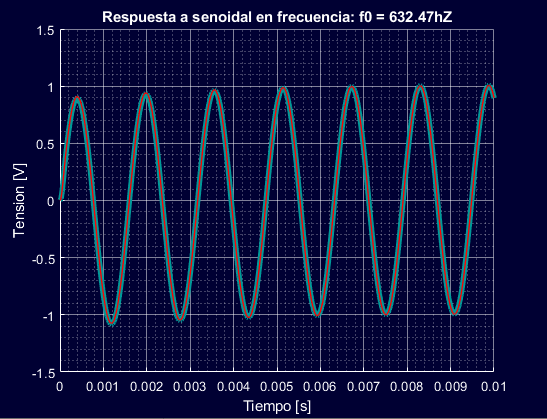
\includegraphics[scale = 0.9]{imagenes/comparacion_senoidal_analitica.png}
    \centering
    \caption{Comparación de la respuesta a senoidal analítica en rojo y la respuesta hallada por Matlab en turquesa}
    \end{figure}
    
    Donde podemos comprobar que coinciden y que luego de un periodo de $4\tau = 0.018$ segundos la respuesta en estado permanente es la misma senoidal de entrada pues alcanza una amplitud de 1. Esto se puede verificar en la respuesta a la senoidal hallada en la sección 2.8
    
    \newpage
    
    \section{Bibliograf'ia}
    
   
        \begin{thebibliography}{9}
        
        \bibitem{}
        \textit{Understanding Poles and Zeros}
        Massachusets Institute of Techonolgy, 2004
        \\\footnotesize\texttt{$http://web.mit.edu/2.14/www/Handouts/PoleZero.pdf$}
        
        \bibitem{} 
        \textit{Analysis of the Sallen-Key architecture}. 
        Texas Instruments, Dallas, Texas, 2002.
        \\\footnotesize\texttt{$www.ti.com/lit/an/sloa024b/sloa024b.pdf?ts$=$1596491525685\&ref_url$=$https\%253A\%252F\%252\\Fwww.google.com\%252F$}
        
        \bibitem{} 
        \textit{LTSpice Tutorial}. 
        Wilfrid Laurier University, 2019 
        \\\footnotesize\texttt{http://denethor.wlu.ca/ltspice/\#vpulse}
        
        \end{thebibliography}
    
    
\end{document}
